Project made using QT Creator in C++\hypertarget{index_about}{}\section{About}\label{index_about}
A simple cross-\/platform steganography project which hides data in images. This project was built using amazing \href{https://qt.io}{\tt Qt Framework} and \href{https://github.com/bricke/Qt-AES}{\tt Q\+A\+E\+S\+Encryption} by \href{https://github.com/bricke}{\tt bricke}. You can read more about project at the \href{waleko.github.io/PictureCrypt}{\tt home page}\hypertarget{index_structure}{}\section{Structure of the project}\label{index_structure}
M\+VC pattern used. Here is a simple project scheme, showing main classes. 
\begin{DoxyImageNoCaption}
  \mbox{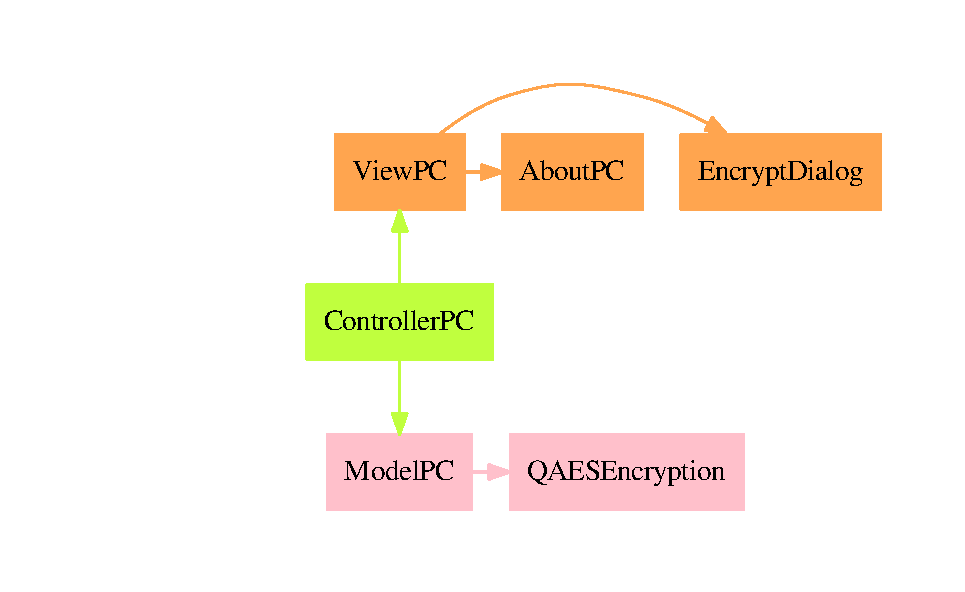
\includegraphics[width=\textwidth,height=\textheight/2,keepaspectratio=true]{dot_structure}}
\end{DoxyImageNoCaption}
\hypertarget{index_ext-use}{}\section{External use}\label{index_ext-use}
You can use \hyperlink{class_model_p_c}{Model\+PC} class separately from View and Control layer. You will need just the src/app/model folder, so these four files\+:


\begin{DoxyItemize}
\item \hyperlink{modelpc_8cpp}{modelpc.\+cpp} 
\item \hyperlink{modelpc_8h}{modelpc.\+h} 
\item \hyperlink{qaesencryption_8cpp}{qaesencryption.\+cpp} 
\item \hyperlink{qaesencryption_8h}{qaesencryption.\+h} 
\end{DoxyItemize}

Then you can just {\ttfamily \#include \char`\"{}modelpc.\+h\char`\"{}} and use A\+PI.\hypertarget{index_use_api}{}\subsection{A\+PI}\label{index_use_api}
Here is are the most important methods\+: 
\begin{DoxyItemize}
\item \hyperlink{class_model_p_c_a271cf9285e32df58ffbfc918e6482bbd}{Model\+P\+C\+::\+Encrypt} 
\item \hyperlink{class_model_p_c_a902abaea4f07995b48c0f2fea6eceb7c}{Model\+P\+C\+::\+Decrypt} 
\end{DoxyItemize}\hypertarget{index_Showcase}{}\subsubsection{Showcase}\label{index_Showcase}

\begin{DoxyCode}
\textcolor{comment}{// Includes}
\textcolor{preprocessor}{#include "\hyperlink{modelpc_8h}{modelpc.h}"}
\textcolor{preprocessor}{#include <QImage>}
\textcolor{preprocessor}{#include <QByteArray>}
\textcolor{preprocessor}{#include <QString>}
\textcolor{preprocessor}{#include <QDebug>} \textcolor{comment}{// just for showcase}

...

\textcolor{comment}{// Basic setup}
QByteArray data(\textcolor{stringliteral}{"some\_file.txt"});
QImage *image = \textcolor{keyword}{new} QImage(\textcolor{stringliteral}{"some\_big\_enough\_image.jpg"});
QString key = \textcolor{stringliteral}{"some\_password"};
\textcolor{keywordtype}{int} bitsUsed = 3; \textcolor{comment}{// must be from 1 to 8}

\textcolor{comment}{// Encrypting}
QString error1, error2;
QImage *normal\_resultImage = \hyperlink{class_model_p_c_a271cf9285e32df58ffbfc918e6482bbd}{ModelPC::Encrypt}(
    data,
    image,
    1, \textcolor{comment}{// normal mode}
    key,
    bitsUsed,
    &error1);
QImage *advanced\_resultImage = \hyperlink{class_model_p_c_a271cf9285e32df58ffbfc918e6482bbd}{ModelPC::Encrypt}(
    data,
    image,
    2, \textcolor{comment}{// advanced mode}
    key,
    bitsUsed, \textcolor{comment}{// not really used here, so put here any number from 1 to 8}
    &error2);

\textcolor{comment}{// Decrypting with given mode}
QString error3, error4, error5, error6;
QByteArray output\_normal = \hyperlink{class_model_p_c_a902abaea4f07995b48c0f2fea6eceb7c}{ModelPC::Decrypt}(
    normal\_resultImage,
    key,
    1, \textcolor{comment}{// normal}
    &error3);
QByteArray output\_advanced = \hyperlink{class_model_p_c_a902abaea4f07995b48c0f2fea6eceb7c}{ModelPC::Decrypt}(
    advanced\_resultImage,
    key,
    2, \textcolor{comment}{// advanced}
    &error4);

\textcolor{comment}{// Decrypting without given mode}
\textcolor{comment}{// PictureCrypt can detect the mode of the image and adapt.}
QByteArray output\_normal\_undefined = \hyperlink{class_model_p_c_a902abaea4f07995b48c0f2fea6eceb7c}{ModelPC::Decrypt}(
    normal\_resultImage,
    key,
    0, \textcolor{comment}{// auto-detect mode}
    &error5);
QByteArray output\_advanced\_undefined = \hyperlink{class_model_p_c_a902abaea4f07995b48c0f2fea6eceb7c}{ModelPC::Decrypt}(
    advanced\_resultImage,
    key,
    0, \textcolor{comment}{// auto-detect mode}
    &error6);

\textcolor{comment}{// Check (better testing with running tests [See section 'Run tests'])}
\textcolor{keywordtype}{bool} data\_good =
    data == output\_normal &&
    data == output\_advanced &&
    data == output\_normal\_undefined &&
    data == output\_advanced\_undefined;
\textcolor{keywordtype}{bool} no\_errors =
    error1 == \textcolor{stringliteral}{"ok"} &&
    error2 == \textcolor{stringliteral}{"ok"} &&
    error3 == \textcolor{stringliteral}{"ok"} &&
    error4 == \textcolor{stringliteral}{"ok"} &&
    error5 == \textcolor{stringliteral}{"ok"} &&
    error6 == \textcolor{stringliteral}{"ok"};
\textcolor{keywordflow}{if}(data\_good && no\_errors)
    qDebug() << \textcolor{stringliteral}{"PASS"};
\textcolor{keywordflow}{else}
    qDebug() << \textcolor{stringliteral}{"FAIL"};
\end{DoxyCode}
\hypertarget{index_license}{}\section{License}\label{index_license}
This software is provided under the M\+IT License\hypertarget{index_contact}{}\section{Contact us}\label{index_contact}
Visit my site\+: \href{https://www.alexkovrigin.me}{\tt https\+://www.\+alexkovrigin.\+me}

Email me at \href{mailto:a.kovrigin0@gmail.com}{\tt a.\+kovrigin0@gmail.\+com}

\begin{DoxyAuthor}{Author}
Alexander Kovrigin (waleko) 
\end{DoxyAuthor}
\begin{DoxyCopyright}{Copyright}
Alexander Kovrigin 2019  
\end{DoxyCopyright}
